\documentclass{article}

% packages
\usepackage[margin=.5in]{geometry}
\usepackage{enumitem}
\usepackage[none]{hyphenat}
\usepackage[dvipsnames]{xcolor}
\usepackage{hyperref}
\usepackage{tikz}
\usepackage{float}

% details
\author{koku17}
\title{Module 1}

% presets
\usetikzlibrary{
	arrows.meta,
	decorations.text
}
\hypersetup{
	hidelinks
}
\pagecolor{black}
\color{white}

% macros
\newcommand{\ctbox}[1]{
	\begin{tabular}{c}
		#1
	\end{tabular}
}
\newcommand{\tbox}[2]{
	\begin{tabular}{#1}
		#2
	\end{tabular}
}
\newcommand{\tpath}[4]{
	\path[
		xshift=#3,
		yshift=#4,
		decorate,
		decoration={
			text along path,
			text={#1},
			text color=white,
			text align=center
		}] #2;
}

\begin{document}
	\pagenumbering{gobble} \maketitle \newpage
	\pagenumbering{roman} \pdfbookmark[1]{Contents}{} \tableofcontents
	\pdfbookmark[1]{List of Figures}{} \listoffigures \newpage
	\pagenumbering{arabic}

	\section{Introduction}
	\subsection{Meaning of Research}
	Research refers to a careful, well-defined (or redefined), objective, and systematic method of search for
	knowledge or formulation of a theory that is driven by inquisitiveness for that which is unknown and useful
	on a particular aspect so as to make an original contribution to expand the existing knowledge base

	\begin{itemize}
		\item Research can be defined as the search for knowledge or as any systematic investigation to
			establish facts.
		\item Research is like a careful and organized journey to find new information or create new knowledge.
		\item It involves setting a clear goal, asking questions, forming hypotheses (educated guesses),
			analyzing data and making sure your conclusions match your initial ideas.
	\end{itemize}

	\noindent \textbf{Example} \\
	Imagine you are curious about why plants in your garden grow differently. Your research could involve
	observing, making guesses (hypothesis), collecting data about sunlight, soil and water, and then figuring
	out why plants grow differently. \newpage

	\subsubsection{Starting Research Cycle}
	The research process (or research cycle) basically begins with a \textbf{practical problem} or an existing
	gap in knowledge or practice. This could be a practical challenge, an unanswered question, or an area that
	needs improvement.

	\begin{figure}[H]
		\centering
		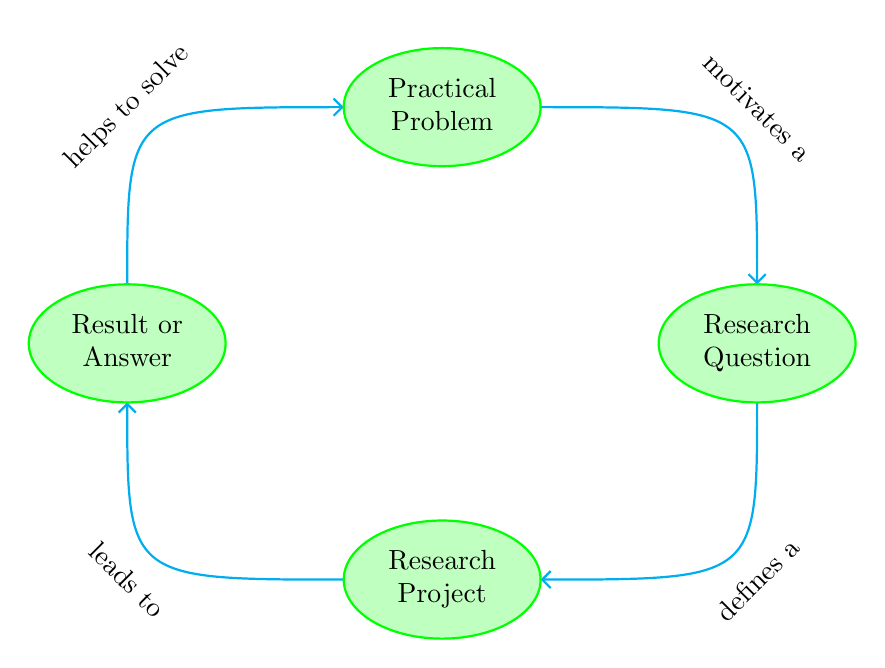
\begin{tikzpicture}
			\draw[thick,-Straight Barb,color=cyan] (1.25,0) .. controls (4,0) .. (4,-2.25);
			\draw[thick,-Straight Barb,color=cyan] (4,-3.75) .. controls (4,-6) .. (1.25,-6);
			\draw[thick,-Straight Barb,color=cyan] (-1.25,-6) .. controls (-4,-6) .. (-4,-3.75);
			\draw[thick,-Straight Barb,color=cyan] (-4,-2.25) .. controls (-4,0) .. (-1.25,0);

			\draw[thick,draw=green,fill=green,fill opacity=.25,text opacity=1]
				(0,0)   ellipse (1.25cm and .75cm) node (1) {\ctbox{Practical \\ Problem}}
				(4,-3)  ellipse (1.25cm and .75cm) node (2) {\ctbox{Research \\ Question}}
				(0,-6)  ellipse (1.25cm and .75cm) node (3) {\ctbox{Research \\ Project}}
				(-4,-3) ellipse (1.25cm and .75cm) node (4) {\ctbox{Result or \\ Answer}}
			;

			\draw
				node[rotate=-45] at (4,0)   {motivates a}
				node[rotate=45]  at (4,-6)  {defines a}
				node[rotate=-45] at (-4,-6) {leads to}
				node[rotate=45]  at (-4,0)  {helps to solve}
			;
		\end{tikzpicture}
		\caption{Research Cycle}
	\end{figure}

	\begin{itemize}
		\item Once the problem is identified, researchers formulate a clear and concise problem statement.
		\item From the formulated problem statement, researchers then develop specific research questions.
		\item Building on the \textbf{research questions}, researchers set clear objectives for the study.
		\item Objectives outline what the research aims to achieve and contribute to solving the identified
			problem.
		\item They serve as a roadmap for the \textbf{research project}.
	
		\item Based on the research questions and objectives, researchers design a methodology to gather
			relevant data and conduct the investigation.
		\item This may involve selecting research methods, data collection techniques, and analytical tools
			suitable for addressing the research questions.
		\item Researchers collect data according to the defined methodology.
	
		\item This data is then analyzed to derive meaningful insights and \textbf{results or answers} to the
			research questions.
		\item The results of the analysis are interpreted in the context of the research questions and
			objectives.
		\item The final step involves translating research findings into practical implications.
		\item This helps to solve the practical problem that one started with in the first place, as shown in
			the following figure.
	\end{itemize}

	\noindent \textbf{Example} \\
	If you notice your plants are not growing well, the problem is the poor plant growth. \\
	Your research question might be, \emph{``What factors affect plant growth in my garden ?"} \newpage

	\subsubsection{Building Background}
	\begin{itemize}
		\item The building up of background for doing good research includes connecting different areas or
			different pieces of knowledge.
		\item The purpose is to prepare the mind for active work as opposed to becoming a repository or an
			encyclopedia.
		\item Research is not just about reading a lot of books and gathering a lot of existing information.
		\item It is about adding our own ideas to what we already know.
		\item It involves critical thinking, analysis, and the generation of new insights.
		\item Research is about asking questions that matter in the real world and then finding answers
			through a careful and organized approach.
		\item It involves systematically exploring, investigating, and understanding topics that are relevant
			to our lives.
		\item The purpose is to prepare the mind for active work as opposed to becoming a repository or an
			encyclopedia.
		\item Research is not just about reading or gathering a lot of existing information.
		\item It is instead adding, maybe small and specific, yet original, contribution to that existing body
			of knowledge.
	\end{itemize}

	\noindent \textbf{Example} \\
	Before fixing your garden, you might learn about soil types, sunlight needs, and plant nutrition. \\
	Instead of just gathering facts(existing information), you aim to contribute something new and specific.

	\subsubsection{Ways of Developing Knowledge}
	The ways of developing and accessing knowledge come in three, somewhat overlapping, broad categories. \\
	They are observation (seeing things), models (simplified descriptions or equations), and processes (methods
	or designs).

	\begin{figure}[H]
		\centering
		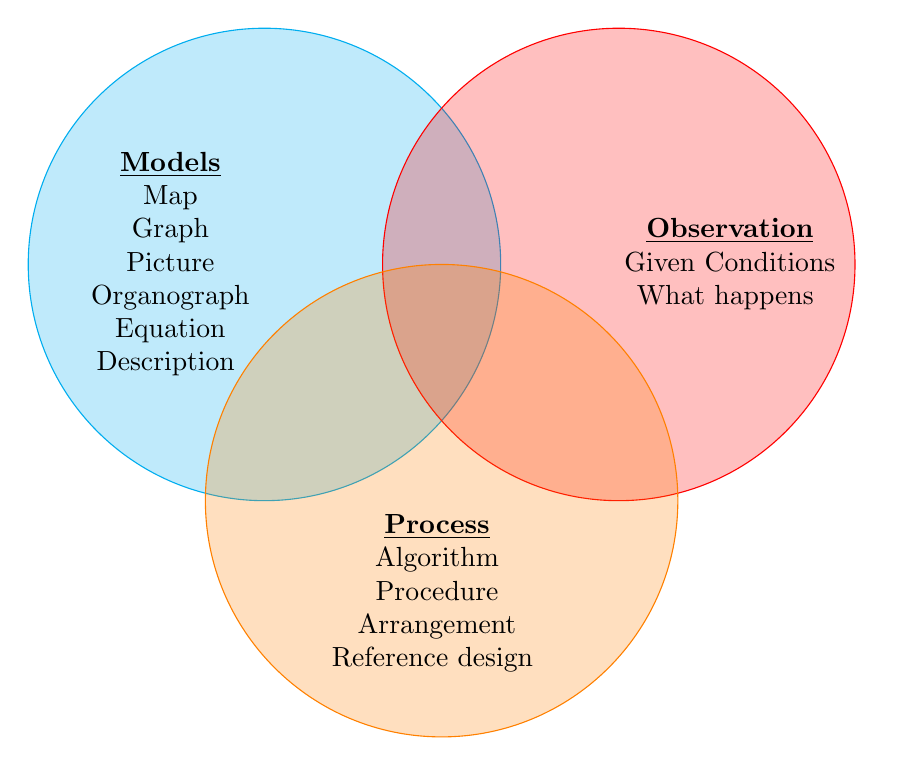
\begin{tikzpicture}[scale=1.5]
			\draw[draw=cyan,fill=cyan,fill opacity=.25,text opacity=1] (0,0) circle (2cm)
				node[left,xshift=.75em] {
					\ctbox{
						\textbf{\underline{Models}} \\
						Map \\ Graph \\ Picture \\ Organograph \\ Equation \\ Description
					}
				};
			\draw[draw=red,fill=red,fill opacity=.25,text opacity=1] (3,0) circle (2cm)
				node[right,xshift=-.75em] {
					\ctbox{
						\textbf{\underline{Observation}} \\
						Given Conditions \\ What happens
					}
				};
			\draw[draw=orange,fill=orange,fill opacity=.25,text opacity=1] (1.5,-2) circle (2cm)
				node[below] {
					\ctbox{
						\textbf{\underline{Process}} \\
						Algorithm \\ Procedure \\ Arrangement \\ Reference design
					}
				};
		\end{tikzpicture}
		\caption{Developing and accessing knowledge}
	\end{figure}

	\begin{enumerate}[label=\textbf{\roman*)}]
		\item \textbf{Observation}
			\begin{itemize}
				\item Observation is described as the most fundamental way to gather information.
				\item It becomes particularly important when the subject being observed is unusual, exciting,
					or challenging to study.
				\item Observation can take various forms, ranging from traditional measurements in a laboratory
					setting to conducting surveys among a group of subjects.
			\end{itemize}
		\item \textbf{Models}
			\begin{itemize}
				\item After making observations, the collected data often needs to undergo some form of
					processing, which leads to the second category of knowledge, which is the ``model".
				\item \textbf{Models} are described as approximated and simplified representations in the form
					of a statistical relationship, a figure, or a set of mathematical equations.
				\item Models help us understand and interpret observed phenomena more abstractly, providing a
					way to analyze and make sense of the data.
			\end{itemize}
		\item \textbf{Processes and Algorithms}
			\begin{itemize}
				\item The final category involves methods for organizing and doing things to achieve a
					specific result.
				\item This category includes processes, algorithms, procedures, arrangements, or reference
					designs.
			\end{itemize}
	\end{enumerate}

	\noindent \textbf{Example : Consider development of a Smartphone} \\
	Engineers observe user interactions with existing smartphones, studying how people use different features,
	how they hold the device, and identifying common issues such as battery life and durability concerns.
	This observation helps engineers understand user behavior and preferences, as well as identify potential
	problems or areas for improvement. \\

	\noindent Based on the observed data, engineers create models to simulate the behavior of various
	smartphone components.
	These models help predict factors like power consumption, signal strength, and heat dissipation,
	influencing design choices. \\

	\noindent Engineers follow a detailed development process for manufacturing the smartphone.
	This involves procedures for designing the circuit board, arranging hardware components such as the
	battery, processor, camera, and sensors within the device, implementing algorithms for software
	functionalities, and adhering to reference designs to ensure compatibility with industry standards.

	\subsubsection{Good Research}
	\begin{itemize}
		\item Good research involves a systematic approach to collecting and analyzing information.
		\item Good research includes systematically collecting and analyzing information.
		\item It goes beyond existing knowledge, attempting to add valuable discoveries.
		\item The research journey in engineering typically starts with a broad research area (i.e. AIML) and
			narrows down to a specific topic (CV), ultimately focusing on a well-defined problem
			(Enhancing accuracy in image recognition systems).
		\item This progression from area to topic to problem showcases the gradual refinement of research focus.
	\end{itemize}

	\noindent \textbf{Example} \\
	In gardening research, after applying your watering schedule, you analyze plant growth data. \\
	If you discover a new and effective way to make plants thrive, you have made an important discovery.

	\subsubsection{Engineering Research}
	\begin{itemize}
		\item In engineering, research involves recognizing, planning, designing, and executing investigations
			to improve knowledge and skills.
		\item Engineering research is the process of developing perspectives and seeking improvements in
			knowledge and skills to enable the recognition, planning, design, and execution of research in a
			wide range of forms relevant for engineering and technology investigations and developments.
		\item In other words, engineering research is a systematic and disciplined process aimed at discovering
			new knowledge or improving existing knowledge in the field of engineering.
	\end{itemize}

	\noindent \textbf{Example} \\
	If you are an engineer wondering why a machine works a certain way, your research might involve studying
	its parts, creating models to understand interactions, and eventually suggesting ways to make it work
	better.

	\section{Objectives of Engineering Research and Motivation in Engineering Research}
	\subsection{Objectives of Engineering Research}
	\begin{itemize}
		\item The primary goal of engineering research is to address new and significant problems.
		\item While the ultimate conclusion is unknown at the start, the process begins with educated guesses
			based on circumstantial evidence, intuition, and imagination.
		\item A guess gives a target to work toward and after initial attempts, it may turn out that the guess
			is incorrect.
		\item Engineering research serves various important objectives, contributing to the advancement of
			knowledge, technology, and societal well-being.
	\end{itemize}

	\subsubsection{Key objectives of engineering research}
	\begin{enumerate}[label=\textbf{\roman*)}]
		\item \textbf{Innovation and Advancement} \\
		Engineering research aims to push the boundaries of current knowledge and technology.
		By exploring new ideas, concepts, and methodologies, researchers seek to innovate and advance the
		field, leading to the development of new technologies and solutions.

		\item \textbf{Problem Solving} \\
		Engineering research often focuses on solving real-world problems.
		Researchers aim to address challenges and issues faced by industries, communities, or individuals,
		seeking practical and effective solutions through the application of engineering principles.

		\item \textbf{Optimization} \\
		Research in engineering aims to optimize existing processes, systems, and products.
		This involves improving efficiency, reducing costs, enhancing performance, and minimizing
		environmental impacts.

		\item \textbf{Knowledge Expansion} \\
		One of the primary objectives of research is to expand the body of knowledge in engineering.
		Through experimentation, analysis, and documentation, researchers contribute to the understanding of
		fundamental principles and phenomena in various engineering disciplines.

		\item \textbf{Interdisciplinary Collaboration} \\
		Many engineering challenges require a multidisciplinary approach.
		Research objectives may involve collaboration between engineers, scientists, and professionals from
		other fields to address complex problems that span multiple domains.

		\item \textbf{Education and Training} \\
		Engineering research contributes to the education and training of future engineers and scientists.
		The dissemination of research findings through publications, conferences, and other channels helps
		educate the next generation of professionals.

		\item \textbf{Technological Transfer}
		Research often leads to the development of new technologies and methodologies.
		The objective is not only to create knowledge but also to transfer this knowledge to industry, enabling
		the practical application of research findings for the benefit of society.

		\item \textbf{Societal Impact} \\
		Many engineering research projects are driven by a desire to have a positive impact on society.
		This could involve improving infrastructure, addressing practices, environmental issues,
		enhancing healthcare technologies, or promoting sustainable.

		\item \textbf{Quality and Safety Improvement} \\
		Engineering research aims to enhance the quality and safe y of products, processes, and systems.
		This is particularly important in fields such as aerospace, healthcare, and transportation, where
		safety standards are crucial.

		\item \textbf{Global Challenges} \\
		Engineering research often addresses global challenges such as climate change, resource scarcity, and
		public health issues. The objective is to contribute to solutions that can have a positive impact on a
		global scale.
	\end{enumerate}

	\subsection{Motivation in Engineering Research}
	Motivation in engineering research plays an important role in driving researchers to explore new
	frontiers, address challenges, and contribute to the advancement of knowledge and technology.
	Motivations can broadly be categorized into intrinsic, extrinsic, and sometimes a blend of both.
	The combination of both intrinsic and extrinsic motivators can shape the overall motivation of individuals
	engaging in engineering research.

	\subsubsection{Intrinsic Motivations}
	Intrinsic motivations refer to the internal factors that drive a person to engage in an activity.

	\begin{enumerate}[label=\textbf{\roman*)}]
		\item \textbf{Curiosity and Intellectual Interest} \\
		Many researchers are motivated by a natural curiosity and a genuine interest in understanding how
		things work.
		Studies have shown that intrinsic motivations like interest, challenge, learning, Meaning and purpose
		are linked to strong creative performance.

		\textbf{Example} \\
		An engineer may be naturally curious about the functioning of renewable energy systems.
		This curiosity drives him to explore innovative approaches to harnessing solar energy, leading to
		research in the development of more efficient solar panels.

		\item \textbf{Personal Fulfillment} \\
		For some researchers, the pursuit of knowledge and the satisfaction of contributing to the greater body
		of human understanding are personally fulfilling.
		The intrinsic rewards of research, such as personal growth and a sense of accomplishment, can be
		powerful motivators.
		Personal motivation for solving unsolved problems, intellectual joy, service to the community, and
		respectability are all driving factors.

		\textbf{Example} \\
		An environmental engineer driven by a sense of purpose to address pollution may engage in research on
		innovative waste management solutions.
		The meaningful impact on the environment serves as a driving force.

		\item \textbf{Passion for Technology} \\
		Individuals with a genuine passion for engineering and technology may find motivation in the joy of
		working with and contributing to the development of advanced technologies.

		\textbf{Example} \\
		An engineer with a deep passion for robotics may initiate research to enhance the capabilities of
		autonomous robots.
		The joy and satisfaction derived from contributing to the field of robotics serve as intrinsic
		motivators.
	\end{enumerate}

	\subsubsection{Extrinsic Motivations}
	\begin{enumerate}[label=\textbf{\roman*)}]
		\item \textbf{Career Development} \\
		Engaging in research can contribute to career advancement in academia, industry, or both.
		Researchers may be motivated by the desire to establish themselves as experts in their field, gain
		recognition, and open up new opportunities for professional growth. Extrinsic motivating factors like
		rewards for good work, such as money, fame, awards, praise, and status, are very strong motivators but
		may block creativity.

		\textbf{Example} \\
		Research outcomes may enable a researcher to obtain a patent, which is a good way to become rich and
		famous, opening up opportunities for career growth and recognition.

		\item \textbf{Competitive Drive} \\
		The desire to be at the forefront of a field or to compete with other researchers and institutions can
		drive motivation.
		The pursuit of excellence and the aspiration to be recognized for outstanding contributions can be
		strong motivating factors.

		\item \textbf{Influences from others} \\
		Influences from others, like collaboration, commitment, and encouragement, are also motivating factors
		in research.

		\textbf{Example} \\
		My friends are all doing research and so should I, or a person that I dislike, be doing well and I want
		to do better.
	\end{enumerate}

	\subsubsection{Mix of Extrinsic and Intrinsic Motivations}
	The following factors would be a mix of extrinsic and intrinsic aspects in Engineering Motivation

	\begin{enumerate}[label=\roman*)]
		\item \textbf{Wanting to do better than what has been achieved in the world} \\
		This is an intrinsic motivation, driven by personal motivation and a desire for self-improvement \&
		excellence, and a sense of internal fulfillment.

		\item \textbf{Improve the state of the art in technology} \\
		The pursuit of advancing technology is typically motivated by an intrinsic interest in innovation,
		curiosity, and the internal satisfaction derived from pushing the boundaries of knowledge and
		capability.

		\item \textbf{Contribute to the improvement of society} \\
		This comes under both intrinsic and extrinsic types of motivation, It arises from an internal sense of
		purpose and the desire to make a positive impact on society and address societal challenges.
		It may also be influenced by external factors such as recognition, social approval, or a sense of duty.
		
		\item \textbf{Fulfillment of the historical legacy in the immediate socio-cultural context} \\
		This is a mixed type of motivation, The fulfillment of a historical legacy may be driven by intrinsic
		factors, such as personal meaning and connection to the historical and cultural context, emphasizing a
		sense of identity and continuity. Simultaneously, external factors like societal expectations or
		recognition may also play a role.
		
		\item \textbf{Government directives and funding opportunities} \\
		This represents a mixed type of motivation, influenced by external factors such as government policies
		and financial incentives.
		The motivation to align research with targeted areas for funding is primarily driven by external
		rewards like financial support.
		Simultaneously, it supports researchers in pursuing projects that align with their personal interests,
		curiosity, and passion for contributing to knowledge and innovation.
		
		\item \textbf{Terms of employment} \\
		This represents an extrinsic type of motivation, Terms of employment, including benefits, salary,
		promotions, or job security, are external factors that can motivate individuals to engage in specific
		activities, including engineering research.
	\end{enumerate}

	\section{Types of Engineering Research}

	\section{Finding and Solving a Worthwhile Problem}
	\subsection{Finding a Research Problem}
	A researcher may start with problems stated by the Supervisor or posed by others that are yet to be solved.
	Alternately, it may involve rethinking basic theories or formulating ideas from provided information or
	need to be formulated or put together from the information provided in a group of papers suggested by the
	Supervisor.
	Research scholars face the task of finding an appropriate problem to begin their research.

	\subsection{Skills Needed}
	Skills required for finding a research problem are crucial but often not explicitly taught.
	Critical thinking about possible implications is important.

	\subsection{Identifying a Problem}
	Once the problem is identified, the process of literature survey and technical reading takes place to
	further ascertain the significance and validity of the intended problem.
	An initial spark is ideally required before the process of literature survey may duly begin.
	The process may involve an initial spark from an oral presentation by somebody which is followed by asking
	questions or introspection provides this perspective oral presentation, asking questions, or introspection.
	Developments in other subjects may produce a tool or a result which has direct implications to the
	researcher's subject and may lead to problem identification.

	\subsection{Attributes or characteristics of a Worthwhile Research Problem}
	Once a potential research problem is identified, the researcher faces the critical task of evaluating its
	worthiness.
	A worthwhile research problem possesses one or more attributes, such as being non-intuitive (something that
	goes against common intuition) or counter-intuitive (does not align with what one might naturally expect
	based on prior knowledge or experience), even to someone familiar with the area.

	\begin{enumerate}[label=\roman*)]
		\item Addresses a topic that the research community has been anticipating.
		\item Simplifies a central part of theory.
		\item Introduces a new result, initiating a new subject or area.
		\item Offers a novel method or enhancements to existing methods with practical applications.
		\item Sometimes, provides a result that stops further work in a particular area.
	\end{enumerate}

	\subsection{Decision to Tackle a Problem}
	The researcher must be thoroughly convinced that the problem is worthwhile before initiating the
	investigation.
	Optimal efforts come when the work is worth doing, and the problem and/or solution has a better chance of
	being accepted by the research community. \\

	\noindent \textbf{It is essential to recognize that not every solved problem needs to be of great
	importance or impact}.
	Sometimes major advancements are made through solutions to small problems dealt with effectively.
	Some problems are universally considered hard and open, and have deep implications and connections to
	different concepts. \\

	\noindent Majority of researchers may not engage with such problems during their careers.
	Hard problems get solved only because people take them seriously as challenging problems and
	\textbf{tackle} them with willingness and with determination.
	Such people have a mindset that embraces complexity and uncertainty in the pursuit of solutions.
	They approach problems with a mindset that welcomes complexity and uncertainty in the quest for solutions.
	\\

	\noindent Even if the attempt to solve a challenging problem is unsuccessful, there might be partial or
	side results that can still fulfill the immediate requirement of generating content for the dissertation.

	\section{Ethics in Engineering Research}
	Ethics in engineering research is focused on the ethical considerations within the research process.
	Ethics refers to a set of rules distinguishing acceptable and unacceptable conduct, distinguishing right
	from wrong.
	Most people learn such norms in their formative years but moral development continues through different
	stages of growth.
	Although everyone recognizes common ethical norms, there can be differences in interpretation and
	application.

	\subsection{Ethical Considerations in Authorship}
	Two simple but significant questions to address the tricky issue of authorship in research are :

	\begin{enumerate}[label=\roman*)]
		\item who should be included as an author
		\item appropriate order of listing authors
	\end{enumerate}

	\noindent In today's interconnected world, the issue of co-authorship is very relevant to all researchers,
	challenging the contributions during different phases of research.
	There are issues around individuals may be actively involved in the research process but may not contribute
	to the drafting phase.
	Moreover, certain universities have imposed restrictions on co-authorship to prevent malpractices.

	\subsection{Distinguishing Research Ethics and Responsible Conduct of Research in Engineering}
	Government bodies, and universities worldwide have adopted certain codes for research ethics.
	There is a common misconception regarding the interchangeable use of two terms i.e Research ethics and
	Responsible Conduct of Research.
	Research ethics and the responsible conduct of research are related but not interchangeable.
	Research ethics looks at the ethical application of research outcomes, while Responsible Conduct of
	Research addresses the ethical considerations in how the research work is undertaken.

	\subsubsection{Research Ethics}
	Research ethics primarily focuses on the moral principles and guidelines governing the conduct of research.
	It focuses on ensuring integrity, honesty, and fairness in the research process.
	Key areas include the treatment of research subjects, confidentiality, data handling, and ethical
	communication of research outcomes.
	In essence, research ethics addresses the ethical implications of the research itself.

	\subsubsection{Responsible Conduct of Research}
	Responsible Conduct of Research is a broader concept that extends beyond the ethical dimensions of the
	research itself.
	It encompasses the entire research process, emphasizing ethical behavior in interactions, collaborations,
	and the dissemination of results.
	RCR aims to maintain high standards of integrity and professionalism throughout the research process.

	\begin{table}[H]
		\centering
		\begin{tabular}{|l|l|} \hline
			\multicolumn{1}{|c|}{Research Ethics} & \multicolumn{1}{|c|}{Responsible Conduct of Research}
			\\ \hline & \\
			\begin{tabular}[t]{p{.45\columnwidth}}
				Research ethics involves moral principles governing the conduct of research. \\
				For example, in engineering, it ensures the fair treatment of participants in a human subjects
				study, protection of intellectual property, and honest reporting of results.
			\end{tabular} &
			\begin{tabular}[t]{p{.45\columnwidth}}
				Responsible Conduct of is a broader concept that extends beyond the ethical dimensions of the
				research itself. \\
				In engineering, this includes maintaining integrity in project management, acknowledging
				collaborator's contributions, and avoiding the fabrication on falsification of data.
			\end{tabular} \\ & \\ \hline & \\
			\begin{tabular}[t]{p{.45\columnwidth}}
				Key areas include the treatment of research subjects, confidentiality, data handling, and
				ethical communication of research outcomes.
			\end{tabular} &
			\begin{tabular}[t]{p{.45\columnwidth}}
				RCR aims to maintain high standards of integrity and professionalism throughout the research
				endeavor. \\
				It involves ethical considerations in how the research work in undertaken, including
				interactions and collaborations.
			\end{tabular} \\ & \\ \hline
		\end{tabular}
	\end{table}

	\section{Ethics in Engineering Research Practice}
	Ethics in engineering research practice extends beyond the laboratory or research setting to encompass the
	ethical challenges faced by engineers in the practical application of their knowledge and skills.

	\subsection{Ethical Concerns in Technological Developments}
	Technological progress in engineering introduces ethical considerations, especially regarding privacy and
	data in surveillance systems.
	Engineering researchers bear the responsibility of making ethical decisions, and they are answerable for
	the consequences arising from their research outcomes.

	\subsubsection{Data Collection and Privacy}
	Ethics is crucial in engineering research, especially when working with data, as it directly influences
	human well-being.
	Research involving data collection, especially personal or sensitive information, requires
	respect for individual's privacy and obtaining informed consent. \\

	\noindent \textbf{Example} \\
	A mobile weather app that requests location data for accurate forecasts.
	Ethical concerns arise if the app shares this data without explicit user consent or uses it for purposes
	beyond weather predictions.

	\subsubsection{Acceptability and Validity}
	Certain practices may be acceptable in specific situations, but the reasons for their unacceptability can
	be valid.
	Engineering ethics serves as our rulebook, offering guidance on determining what is ethically acceptable
	and what is not, providing a framework for responsible data use. \\

	\noindent \textbf{Example} \\
	The use of facial recognition in smartphones for unlocking devices might be acceptable for convenience, but
	concerns arise if the technology lacks accuracy and wrongly denies access to users based on facial features.

	\subsection{Ethical Decision-Making in Technological Choices}
	Engineering research is closely interconnected with ongoing technological developments, and researchers
	make numerous choices that hold ethical significance, influencing the impact of technology in various ways.

	\subsubsection{Setting Ethical Requirements}
	At the outset of a project, engineering researchers can shape the effects of the developed technology by
	establishing ethically sound requirements. This initial step sets the stage for the responsible
	technological advancements. \\

	\noindent \textbf{Example} \\
	Engineers working on smart home devices may set ethical requirements for user privacy, ensuring that
	devices like voice-activated assistants only record and transmit data when explicitly activated by users.

	\subsubsection{Influencing Through Design}
	Influence may also be applied by researchers through design, which is a process that translates the
	requirements into a blueprint to fulfill those requirements.
	During the design process, decision is to be made about the priority in importance of the requirements
	taking ethical aspects into consideration. \\
	
	\noindent \textbf{Example} \\
	In the design of automobiles, engineers may prioritize safety features such as collision avoidance systems
	and advanced driver assistance.
	Ethical considerations involve protecting occupants and other road users from potential accidents.
	
	\subsubsection{Choosing Alternatives}
	Throughout the research journey, engineering researchers have to choose between different alternatives
	fulfilling similar functions, considering their ethical implications. \\

	\noindent \textbf{Example} \\
	When developing packaging materials, engineers might choose between traditional plastics and biodegradable
	alternatives.
	Ethical considerations include the environmental impact and long-term sustainability of each option.

	\subsection{Minimizing Unintended Consequences}
	Research outcomes can have unintended and adverse side effects.
	It is important for researchers to ethically address these issues by minimizing the hazards and risks
	associated with their technologies.
	This involves considering safer alternatives, incorporating inherent safety features in designs,
	implementing safety factors, utilizing multiple independent safety barriers, and establishing supervisory
	mechanisms to take control if the primary process fails.
	This commitment to safety demonstrates a careful approach to mitigating potential negative consequences
	from research outcomes. \\

	\noindent \textbf{Example} \\
	Agricultural engineers developing autonomous farming machinery consider unintended consequences, such as
	potential impacts on employment in rural communities.
	Ethical considerations involve implementing strategies to support affected workers and communities.

	\section{Types of Research Misconduct}
	Engineering research should be undertaken with the primary goal of advancing the current state-of-the-art
	technologies.
	Research integrity plays a crucial role in achieving this objective and involves fair dealings with others,
	honesty in presenting methods and results, and replication of findings whenever possible to minimize errors.
	Additionally, upholding the welfare of research subjects, ensuring laboratory safety, and addressing other
	ethical considerations are integral aspects of research integrity.
	In order to prevent mistakes and enhance the quality of research, peer reviews should take place before the
	research output is published. \\
	
	\noindent To prevent errors and enhance the quality of research, it is imperative to subject research
	outputs to peer reviews before publication.
	This practice guarantees that the research undergoes thorough examination by subject-matter experts,
	contributing to the overall reliability and credibility of the research findings.

	\noindent Serious deviations from accepted conduct is construed as research misconduct. \\
	Different types of research misconduct are :

	\subsection{Fabrication (Illegitimate Creation of Data)}
	This involves the act of creating data or experiments with preconceived notions about the expected
	conclusions.
	This unethical practice may arise when there are time constraints imposed by supervisors or customers,
	leading researchers to generate data rather than waiting for genuine results. \\

	\textbf{Example}
	Imagine a student conducting a science experiment on the growth of plants under different light conditions.
	Due to a lack of time, the student decides to fabricate the data by recording measurements that were never
	actually taken.
	The fabricated data might show consistent and impressive growth differences between plants subjected to
	various light conditions.
	In this case, the fabrication involves making up experimental results instead of honestly recording the
	actual outcomes of the plant growth experiment.
	This kind of behavior is unethical and goes against the principles of honesty and integrity in research.

	\subsection{Falsification (Inappropriate Alteration of Data)}
	Falsification involves the inappropriate alteration of data or experiments, including misrepresentation,
	misinterpretation, or illegitimate changes to support a desired hypothesis.
	This unethical practice occurs even when the actual data obtained from experiments indicate a different
	outcome.
	Falsification undermines the credibility and reliability of scientific research by presenting distorted
	information to align with a preconceived notion or agenda.

	\subsection{Consequences of Fabrication and Falsification}
	Negative impacts of fabrication and falsification include :

	\subsubsection{Percolation of False Data}
	When researchers engage in falsification or fabrication, it hampers engineering research, and inaccurate
	results (conclusions) may find their way (percolate) into published literature.
	This compromises the reliability of existing knowledge and can mislead other researchers who rely on this
	information for their work.

	\subsubsection{Wrecking Trustworthiness}
	Unethical practices wreck the trustworthiness of individuals (researchers) involved, damaging their
	reputation.

	\subsubsection{Additional Costs}
	Discovering falsification or fabrication often requires extensive investigations and corrective actions,
	leading to additional financial burdens.

	\subsubsection{Impeded Progress and Delays in Technical Advancement}
	Unethical practices, like falsification and fabrication, slow down research progress by injecting false
	information into the body of knowledge. This misguides other researchers, leading to actual delays in
	technical advancement.

	\subsubsection{Hurt to Honest Researchers}
	Fabrication and falsification create a challenging environment for honest researchers.
	When dishonest or misleading data is already published due to misconduct, it can set a false standard.
	Honest researchers may face challenges in getting their legitimate work recognized and published if it
	falls short of the falsely elevated standards created by misconduct.

	\subsubsection{Publication Barriers}
	The presence of fraudulent or manipulated data in the published literature can create barriers for honest
	researchers.
	This can make it harder for legitimate research to be accepted and published.

	\subsubsection{Establishment of Misconduct}
	Until misconduct is established and proven, the fraudulent data may remain in the published literature.
	This process can take time and may involve investigations and retractions.
	During this period, the misleading information continues to influence the research community.
	The retraction may not fully erase the impact of the false data on the scientific community.

	\noindent Engineering researchers are often perceived as objective truth seekers.
	They can prevent misconduct by independently reproducing results whenever they are interested in doing
	further work on published material, which is likely to be part of their literature survey.

	\subsection{Plagiarism}
	Plagiarism is defined as the act of using or reusing someone else's work, including text, data, tables,
	figures, illustrations, or concepts, without proper attribution.
	It involves presenting the work as if it were one's own without explicit acknowledgment.
	The concept of self-plagiarism occurs when researchers verbatim copy or reuse their own previously
	published work without appropriate citation. This practice is considered unacceptable in scientific
	literature.

	\subsubsection{Challenges of Internet Availability}
	The increasing availability of scientific content on the internet may encourage plagiarism in some cases,
	but also enables detection of such practices through automated software packages designed to identify
	similarities between texts.

	\subsubsection{Detection of Plagiarism}
	How are supervisors, reviewers or editors alerted to plagiarism ?

	\begin{itemize}
		\item Original author comes to know and informs everyone concerned.
		\item Reviewers might discover plagiarism during the review process.
		\item Readers conducting research may come across plagiarized content in articles or books.
	\end{itemize}

	\subsubsection{Plagiarism Detection Tools}
	The availability of both free and paid plagiarism detection tools, often accessible through institutional
	licenses, offers a way to assess the originality of written content, it is important to note that these
	tools provide a similarity score,indicating the level of similarity between published and unpublished
	content, rather than a conclusive identification of plagiarism. A similarity score is not conclusive
	evidence of plagiarism, it only serves as a metric for assessing similarity.

	\noindent However, a low similarity score doesn't guarantee that the document is plagiarism free.
	It requires human evaluation to determine whether the content has been plagiarized or not.
	Additionally, it is essential to consider individual scores of sources rather than just the overall
	similarity index.
	Setting a maximum allowable similarity index may be insufficient in utilizing the tool effectively.
	This is because certain types of plagiarism, such as patchwork plagiarism, where sections of text are
	strategically rearranged, can be more challenging to detect through automated tools.

	\subsubsection{Ethical Writing Practices}
	To avoid a high similarity count, researchers can use relevant published content by rephrasing or
	summarizing the content in their own words. This maintains the original meaning without replicating the
	original text.
	Whenever using ideas, concepts, or findings from other sources, cite them appropriately.
	This gives credit to the original authors and demonstrates transparency in acknowledging the use of
	external information.
	It is important to note that citing a source does not justify verbatim copying.
	A researcher should practice writing in such a way that the reader can recognize the difference between the
	ideas or results of the authors and those that are from other sources.

	\subsection{Other Aspects of Research Misconduct}
	\subsubsection{Deception and Damage (Fraudulent Practices)}
	Serious deviations from accepted conduct could be construed as research misconduct.
	When there is both intentional deception (misleading actions) and damage (negative consequences), the
	actions are officially recognized as fraudulent, and the term ``research misconduct" is often used to
	describe such behavior.
	Such ethical violations are likely to be discovered or exposed over time sooner or later.

	\subsubsection{Simultaneous Submission}
	Engaging in practices that violate publication policies can be considered research misconduct.
	Simultaneous submission of the same article to two different journals violates publication policies.

	\subsubsection{Handling Mistakes in Published Content}
	If a researcher discovers mistakes in their published work and fails to report or correct them, it may be
	viewed as a form of research misconduct, unless a researcher takes responsibility for the accuracy of their
	work, acknowledges the mistake, and is motivated to contribute a corrected version.

	\section{Ethical Issues Related to Authorship}
	Academic authorship involves communicating scholarly work and establishing priority for their discoveries
	and building peer reputation.
	It also comes with an intrinsic burden of accepting responsibility for the contents of the work, serving as
	the primary basis for evaluation in areas such as employment, promotion, and other honors.

	\noindent Here are some common ethical issues related to authorship :
	
	\subsection{Gift or Guest Authorship}
	Including ``guest" or ``gift" authors, where co-authorship is granted to someone with little or no
	contribution to the work, is misleading and unethical.
	This practice dilutes the contributions of those who did the actual work, artificially enhances the
	credentials of the listed authors, and raises concerns about possible research misconduct.

	\subsection{Career-Boost Authorship}
	Sometimes, the primary author may grant co-authorship in a suspicious way to a junior faculty member or a
	student with the intention of enhancing their chances of employment or promotion.
	This practice is referred to as career-boost authorship.
	This may misrepresent contributions, weaken or diminish the integrity of authorship, and be considered
	unethical manipulation for personal gain.

	\subsection{Career-Preservation Authorship}
	This malpractice, termed ``career-preservation authorship", involves adding department heads, deans, or
	other administrators as coauthors in exchange for benefits or maintaining a ``good relationship".
	In such cases, the principal author benefits from a favorable relationship with superiors, while the
	administrator gains authorship credits without fulfilling the necessary work for it, resulting in a
	mutually beneficial arrangement.
	This raises concerns about fairness, transparency, and the actual contributions of individuals listed as
	authors.

	\subsection{Ghost Co-authorship}
	Sometimes, an actual contributor may choose not to be included in the list of authors due to an undisclosed
	conflict of interest (personal or financial) within the organization or other reasons.
	Such instances of co-authorship are referred to as ghost co-authorship.
	This lack of transparency can compromise the integrity and credibility of the research process and findings.
	Full disclosure of all individuals engaged in the research is essential to enable a comprehensive
	evaluation based on both the research findings and an assessment of potential influences arising from
	conflicts of interest.

	\subsection{Reciprocal Authorship}
	In this form of questionable authorship, researchers may include each other as coauthors in a reciprocal
	gesture, often without genuine collaboration.
	The inclusion is based on mutual agreements with an expectation of shared benefits or outcomes.
	In some cases, there might be minimal collaboration, limited to basic tasks such as reading and editing.
	This practice lacks genuine engagement in thoroughly reviewing the work, potentially diminishing the
	credibility of authorship and the research itself.

	\subsection{Misrepresentation of Sole Authorship}
	Some authors try to present their work as solely authored, even when they depend on significant
	contributions from others.
	They choose to acknowledge those contributions only in the form of a general acknowledgment.
	This approach misrepresents the true extent of the contributions made by those not listed as authors.
	In this case, the unrecognized contributors are then unavailable to readers for additional clarification or
	explanation about their role in the research.

	\subsection{Authorial Accountability}
	All listed authors have full responsibility for all contents within a research article, and so naturally,
	they should also be made aware of a journal submission by the corresponding author.
	Obtaining consent from all authors regarding the content and submission of the paper is essential.
	All listed authors are responsible for the content, but determining individual accountability can be
	challenging.
	If one author commits misconduct, it is unclear to what extent other coauthors are responsible.
	Establishing a method to quantify individual contributions would be beneficial in appropriately recognizing
	and assessing the degree of associated accountability for each coauthor.

	\subsection{Double Submission}
	Double submission is an important ethical issue related to authorship, which involves the submission of a
	paper to two forums simultaneously.
	This practice is motivated by the desire to enhance the possibility of publication and potentially reduce
	the time to publication.
	This practice violates the principle of publishing original work, as reputable journals discourage double
	submissions to maintain the integrity of the publication process.
	Reputable journals aim to publish original papers - ones that have not been previously published
	elsewhere and strongly discourage double submission.
\end{document}
